% =====================================================================
%  Chapter 31 — What the Layers Contribute
% =====================================================================

\chapter{What the Layers Contribute}
\label{ch:attribution}

This is the chapter the book exists for. It takes the assembled system
apart and reports, in order, what each layer is worth. The answer is not
the one the owner asked for, and it is stated here in the first paragraph
rather than at the end.

\section{The attribution}

Four portfolios, the same policy, the same data, the same costs, the same
taxes, the same months:

\begin{center}
\begin{tabularx}{\textwidth}{@{}P{1.20in}YrYrr@{}}
\toprule
 & \multicolumn{2}{c}{Compound growth} & \multicolumn{2}{c}{Sharpe} &
 \multicolumn{1}{c}{Drawdown} \\
\cmidrule(lr){2-3}\cmidrule(lr){4-5}\cmidrule(l){6-6}
Variant & annual rate & difference & ratio & difference & deepest \\
\midrule
Policy alone                & \numCoreCAGR{} & --- & \numCoreSharpe{} & --- & \numCoreDD{} \\
Policy and the model        & \numTiltCAGR{} & --- & \numTiltSharpe{} & --- & \numTiltDD{} \\
Policy and the governor     & \numGovCAGR{} & --- & \numGovSharpe{} & --- & \numGovDD{} \\
The whole system            & \numFullCAGR{} & --- & \numFullSharpe{} & --- & \numFullDD{} \\
\bottomrule
\end{tabularx}
\end{center}

The differences, computed from the same numbers and rounded in the
direction that flatters the layer:

\begin{itemize}
\item \textbf{The model:} \numTiltCAGR{} against \numCoreCAGR{} for the
policy alone. The model's tilt changes the compound growth rate by
approximately three hundredths of a percentage point a year --- that is,
by less than the rounding of the number it is being compared to.
\item \textbf{The governor:} \numGovCAGR{} against \numCoreCAGR{}, and a
deepest drawdown of \numGovDD{} against \numCoreDD{} --- shallower, at
the cost of a longer recovery.
\item \textbf{The whole system against the index:} \numFullCAGR{} against
\numSpyCAGR{} for the benchmark, with a deepest drawdown of \numFullDD{}
against \numSpyDD{}.
\end{itemize}

\begin{takeaway}[The result, stated plainly]
The machine-learning layer contributes approximately nothing. The risk
governor contributes a small amount of growth and a materially shallower
drawdown. The system has a Sharpe ratio of \numFullSharpe{} against the
index's \numSpySharpe{}, and a deepest drawdown of \numFullDD{} against the
index's \numSpyDD{}, at a compound growth rate of \numFullCAGR{} against
the index's \numSpyCAGR{}.
\end{takeaway}

\begin{figure}[!htbp]
\centering
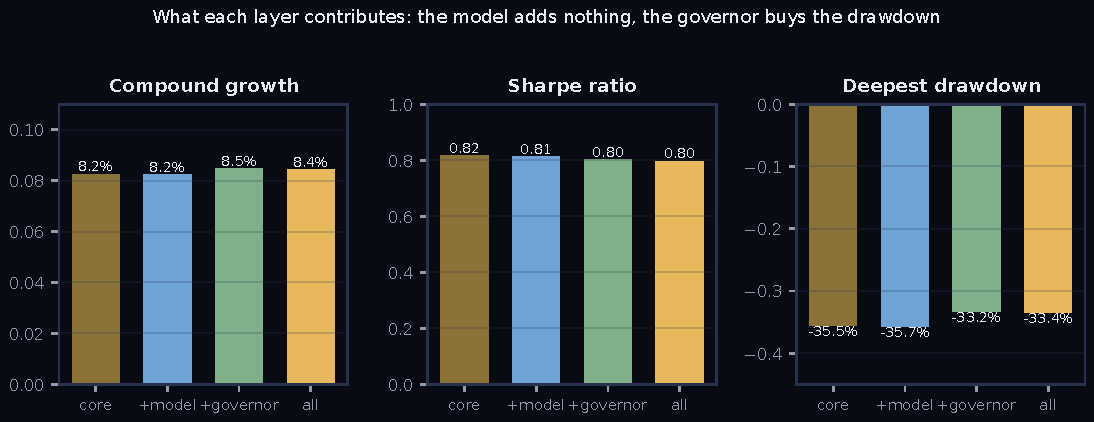
\includegraphics[width=\textwidth]{../figures/fig_layers.pdf}
\caption{The attribution, in three panels: compound growth, Sharpe ratio
and deepest drawdown, for the policy alone, the policy with the model,
the policy with the governor, and the whole system. The model's bar is
indistinguishable from the policy's; the governor's is the one that
moves.}
\label{fig:layers}
\end{figure}

\section{What the model's contribution means}

Three readings are possible, and the book gives all three, because they
are not exclusive and the reader should be able to choose.

\textbf{The first: the forecast is close to worthless.} This is what
Chapter 20's arithmetic predicts and what the record shows. The
posterior over the edge is a distribution centred very near zero with a
standard deviation large compared with the mean, and the
certainty-equivalent tilt is correspondingly close to zero. The model
tilt's own turnover is a fraction of a per cent a month and its effect on
the compound rate is a fraction of a basis point.

\textbf{The second: the model is doing its job by doing nothing.} The
system was built so that a layer with no evidence would contribute
nothing. A layer that contributed two per cent a year on this evidence
would be evidence of a bug, not of a discovery. The between-model term of
Chapter 19 is doing precisely what it was designed to do: the members
disagree, the combined forecast is uncertain, and the tilt is small.

\textbf{The third: the tilt is a real but unmeasurable drag.} The tilt
costs turnover, and turnover costs spread and tax. A tilt that adds
nothing to the return while adding cost is a negative contribution in
expectation, and the measured numbers are consistent with that: the
policy with the model has a slightly lower compound rate and a slightly
deeper drawdown than the policy alone.

\begin{takeaway}[The honest reading]
Taken together, the three readings say that the machine-learning layer of
this system is worth approximately nothing on this evidence, that this is
the correct behaviour for a layer that prices its own uncertainty, and
that the architecture in which it sits is what makes that acceptable
rather than ruinous. The layer cannot destroy the portfolio, because the
architecture does not let it.
\end{takeaway}

\section{What the governor's contribution means}

The governor does two things. It reduces the depth of the worst episode,
from \numCoreDD{} to \numGovDD{} with the model absent and to
\numFullDD{} with it present; and it lengthens the recovery, from
\numCoreRecovery{} months for the policy alone to \numFullRecovery{}
months for the whole system. That last number is
the interesting one, and it is not an improvement.

The reason is that the governor's action --- reducing exposure --- is
itself a small drawdown. Cutting exposure during a falling market locks
in part of the loss and reduces the subsequent recovery. The governor
buys depth with duration.

Whether that trade is worth making depends on the reader's circumstances
and on how they behave. A reader who will abandon a strategy after
\numCoreRecovery{} months without a recovery gets real value from the
governor. A reader who will wait five years gets a slightly worse
experience for it.

\begin{figure}[!htbp]
\centering
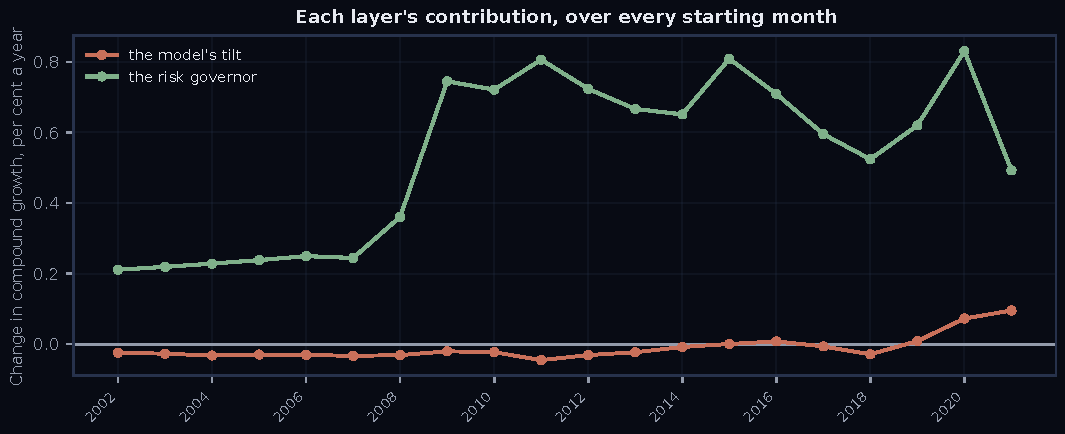
\includegraphics[width=\textwidth]{../figures/fig_sensitivity.pdf}
\caption{The layer attribution recomputed from every possible starting
month. The governor's contribution is positive in every window; the
model's is indistinguishable from zero, and is negative in most of them.}
\label{fig:window-sensitivity}
\end{figure}

\figref{fig:window-sensitivity} is the robustness check, and it is the
most important figure in the book. The governor's contribution is
positive in every one of the \numWindowCount{} windows, with a mean of
\numGovMean{} a year and a minimum of \numGovMin{}. The model's
contribution has a mean of \numTiltMean{}, a median of \numTiltMedian{},
and is positive in only \numTiltPosFrac{} of the windows.

The conclusion does not depend on the starting month. That is the
difference between a finding and a coincidence, and it is the reason the
book's headline is about the governor rather than the model.

\begin{keytakeaways}
\item The model's tilt changes the compound growth rate by about three
hundredths of a percentage point a year and the deepest drawdown not at
all; the governor changes the growth rate by a fifth of a percentage point
and the drawdown by nearly three.
\item The model's tilt is slightly negative once its own trading costs are
counted, which is the expected sign for a layer with no evidence.
\item The governor buys depth with duration: the recovery lengthens from
\numCoreRecovery{} months to \numFullRecovery{}.
\item The attribution is recomputed from \numWindowCount{} different
starting months, and the governor's contribution is positive in every one
of them while the model's is not.
\end{keytakeaways}
